% !TEX root = emba_2027_ouverture.tex
% Compiler depuis EMBA : latexmk -pdf emba_2027_ouverture.tex
\documentclass[aspectratio=169]{beamer}
\makeatletter
\def\input@path{{../latex-common/}}
\makeatother
% ============================================================================
% HEC Montréal MBA -- ECON50803: Environnement macroéconomique
% Shared Beamer Preamble
% ============================================================================
% Loads jfb-teaching-slides.sty from latex-common (sibling repo) for the full
% teaching Beamer aesthetic: Fira Sans fonts, HEC palette, titleframe /
% sectionframe, box envs (keyinsight, bizimplication, warning, defbox,
% exercise), newspaper headlines, backup slides, TikZ styles for AD-AS and
% supply/demand diagrams.
%
% Course-specific configuration, project paths, and overrides live below.
% ============================================================================

\usepackage{jfb-teaching-slides}

% --- Course metadata (drives the footer) ------------------------------------
\jfbcoursename{ECON 50803}
\jfbcoursetitle{Environnement macroéconomique}
\jfbinstitution{HEC Montréal}

% --- Project paths ----------------------------------------------------------
\graphicspath{{../Figures/}}
\newcommand*\includetables[1]{\input{../Tables/#1.tex}}

% --- Shared closing roadmap -----------------------------------------------
% The argument is the session just completed. On the white slide background,
% HECnavy!40 gives completed themes the appearance of 40% opacity.
\newcommand{\coursethemestyle}[3]{%
   \ifnum#1>#2\relax
      \textcolor{HECnavy}{#3}%
   \else
      \textcolor{HECnavy!40}{#3}%
   \fi
}
\newcommand{\courseroadmap}[1]{%
   \begin{frame}{Les thèmes du cours}
      \renewcommand{\arraystretch}{1.4}
      \centering
      \small
      \begin{tabularx}{\textwidth}{>{\bfseries\raggedright\arraybackslash}X >{\raggedright\arraybackslash}p{0.40\textwidth}}
         \toprule
         \textbf{Question centrale} & \textbf{Séance} \\
         \midrule
         \coursethemestyle{1}{#1}{Comment mesurer la production, les prix et le niveau de vie\,?} & \coursethemestyle{1}{#1}{S1 : Mesurer l'économie} \\
         \coursethemestyle{2}{#1}{Pourquoi certains pays sont-ils plus riches que d'autres\,?} & \coursethemestyle{2}{#1}{S2 : Croissance de long terme} \\
         \coursethemestyle{3}{#1}{Qu'est-ce qui détermine l'emploi, les salaires et l'investissement\,?} & \coursethemestyle{3}{#1}{S3 : Marchés du travail et du capital} \\
         \coursethemestyle{4}{#1}{Pourquoi l'économie connaît-elle des hauts et des bas\,?} & \coursethemestyle{4}{#1}{S4 : Cycles économiques} \\
         \coursethemestyle{5}{#1}{Pourquoi et comment combattre les récessions\,?} & \coursethemestyle{5}{#1}{S5 : Politique monétaire et budgétaire} \\
         \bottomrule
      \end{tabularx}
   \end{frame}
}

% --- TikZ style overrides (preserve pre-migration visual choices) ----------
% The shared jfb-teaching-slides.sty defines stronger defaults (e.g.
% supply/demand in HECnavy, eqpoint default HECgreen). Keep the original
% ECON50803 overrides here so existing slides render unchanged.
\tikzset{
   supply/.style     = {very thick},
   original/.style   = {HECgray, thick, dashed},
   refline/.style    = {thin, dashed, HECgray},
   shiftarrow/.style = {very thick, -Stealth},
   eqpoint/.default  = HECnavy,
   eqfaded/.style    = {fill=HECgray, draw=HECgray, opacity=0.4},
   potline/.style    = {HECgreen, thick, dashed},
   econbrace/.style  = {decorate, decoration={brace, amplitude=6pt, mirror}, thick},
   pointlabel/.style = {font=\small},
   annotlabel/.style = {font=\small},
}

% --- Exam-relevance tag -----------------------------------------------------
% Enable the stars per session with \showexamtagstrue after loading this file.
\newif\ifshowexamtags
\showexamtagsfalse
\usetikzlibrary{shapes.geometric}
\newcommand{\examtag}{%
   \ifshowexamtags%
      \AddToHookNext{shipout/foreground}{%
         \put(\dimexpr\paperwidth - 0.5cm\relax,-0.65cm){%
            \makebox(0,0)[rt]{%
               \tikz \node[star, star points=5, star point ratio=2.25,
                           fill=HECcoral, inner sep=1.6pt] {};%
            }%
         }%
      }%
   \fi%
}

\graphicspath{{../Slides/Figures/}}
\jfbcoursename{EMBA McGill–HEC Montréal}
\jfbcoursetitle{Environnement macroéconomique et stratégie}
\jfbinstitution{HEC Montréal}
% La page titre partagée se termine par « MBA ». Adapter uniquement ce libellé.
\patchcmd{\titleframe}{\enspace MBA}{\enspace EMBA}{}{\PackageError{emba}{Vérifier le libellé de la page titre}{}}
\title{L’environnement macroéconomique\\au cœur des décisions stratégiques}
\author{Jean-Félix Brouillette}
\date{28 janvier 2027}

\begin{document}

% 9 h – 9 h 07 | Ouverture de L’essentiel du MBA, avec la grille de Vincent appliquée à la manchette sur le pétrole.
% 1
\titleframe

% 2
\begin{frame}{Présentation}
   \begin{columns}[c]
      \begin{column}{0.35\textwidth}
         \begin{center}
            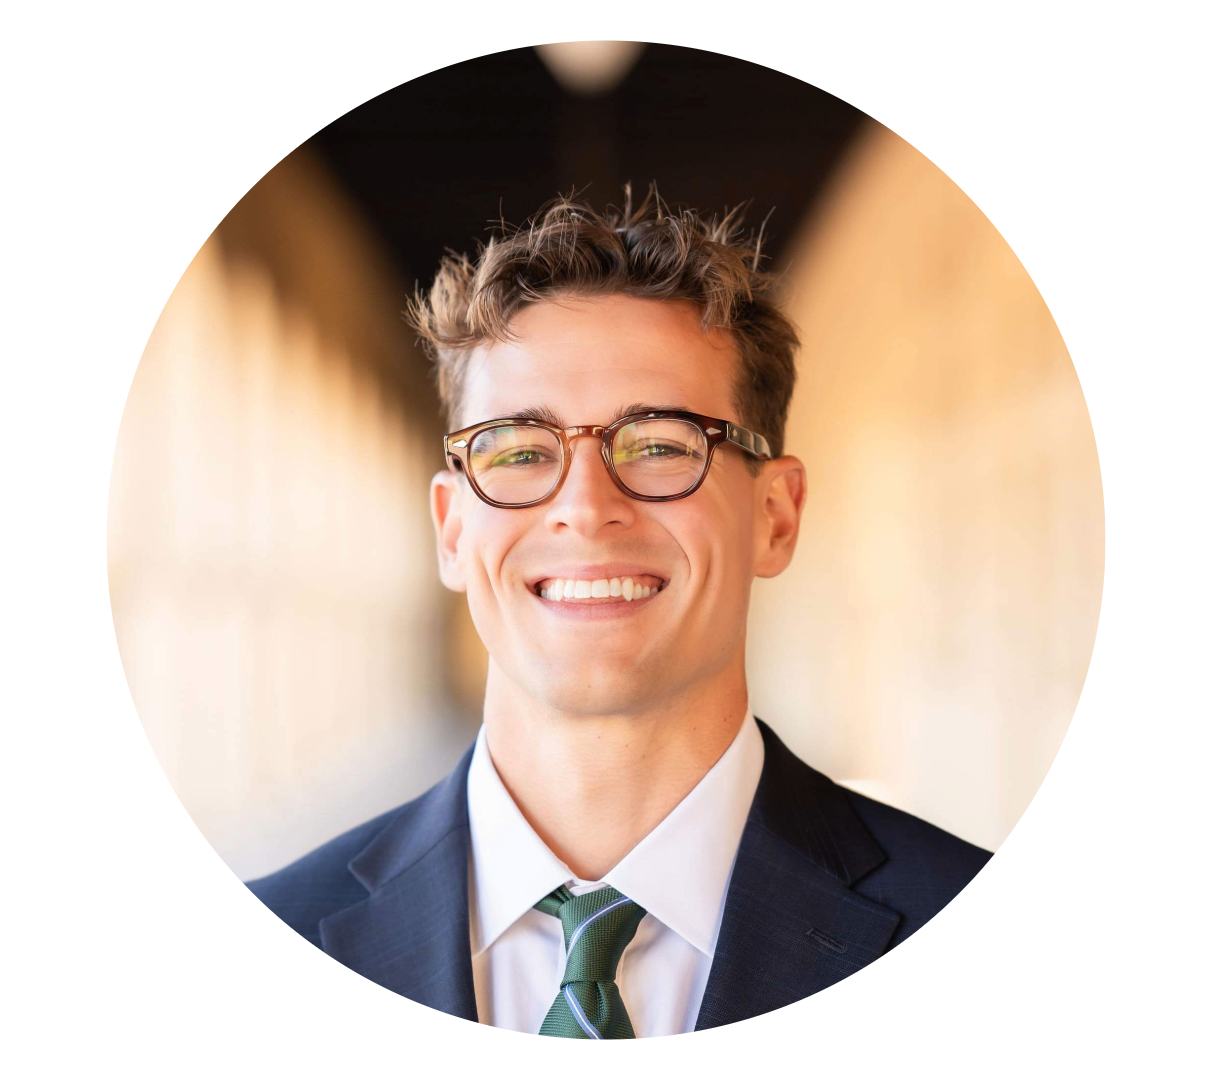
\includegraphics[width=1.0\textwidth]{headshot}
         \end{center}
      \end{column}
      \hspace{-1cm}
      \begin{column}{0.65\textwidth}
         \textbf{Jean-Félix Brouillette} \\[0.15cm]
         Professeur adjoint en économie appliquée \\[0.3cm]
         {\small B.A.A.\ et M.Sc.\ en économie, HEC Montréal \\
         Ph.D.\ en économie, Stanford University} \\[0.3cm]
         \begin{itemize}
            \setlength\itemsep{0.15cm}
            \item Courriel : {\small \href{mailto:jean-felix.brouillette@hec.ca}{jean-felix.brouillette@hec.ca}}
         \end{itemize}
      \end{column}
   \end{columns}
\end{frame}

% 3 | Mosaïque de six manchettes de L’essentiel du MBA.
\begin{frame}{Un monde complexe et incertain}
  \begin{tikzpicture}[remember picture,overlay]
    \setcounter{newshl}{0}
    \newsheadline[globeandmail]{The Globe and Mail}{\href{https://www.theglobeandmail.com/business/article-bank-of-canada-raises-interest-rate-october-2026/}{\guillemotleft~BoC hikes rate to 2.5\% to contain oil-price shock~\guillemotright}}
    \newsheadline[ft]{Financial Times}{\href{https://www.ft.com/content/9cb63980-cd43-419d-a7e5-42039b9fd01e?syn-25a6b1a6=1}{\guillemotleft~The multiplying risks of financing data centres~\guillemotright}}
    \newsheadline[bloomberg]{Bloomberg}{\href{https://www.bloomberg.com/news/articles/2026-09-23/us-treasury-five-year-yields-breach-5-for-first-time-since-2007}{\guillemotleft~US Bond-Market Slide Deepens, Pushing Yields to Two-Decade Highs~\guillemotright}}
    \newsheadline[reuters]{Reuters}{\href{https://theedgemalaysia.com/node/820812}{\guillemotleft~Oil rises as investors weigh supply threats~\guillemotright}}
    \newsheadline[lapresse]{La Presse}{\href{https://www.lapresse.ca/affaires/economie/2026-10-06/etude-de-la-banque-du-canada/la-replique-tarifaire-du-canada-alimente-l-inflation.php}{\guillemotleft~La réplique tarifaire du Canada alimente l'inflation~\guillemotright}}
    \newsheadline[ledevoir]{Le Devoir}{\href{https://www.ledevoir.com/economie/1015754/economie-quebecoise-perdu-49-000-emplois-septembre}{\guillemotleft~L'économie québécoise a perdu 49\,000 emplois en septembre~\guillemotright}}
    \node[anchor=south west,text=HECtext!70,font=\scriptsize] at ([xshift=1.2cm,yshift=.65cm]current page.south west)
      {Manchettes d’août à octobre 2026};
  \end{tikzpicture}
  \note{Laisser le groupe parcourir les six manchettes. Relever celle de Reuters sur le pétrole. Comment une dépense de plus à la pompe se répercute-t-elle ailleurs dans l’économie\,? Introduire ce passage de l’individu au groupe avec l’exemple du hockey.}
\end{frame}

% 4 | Texte de l’ouverture initiale. Les flèches relient les deux échelles de décision.
\begin{frame}{Qu’est-ce que la macroéconomie\,?}
  \centering
  \begin{tikzpicture}[
    definition/.style={rounded corners=5pt,align=left,text width=5.5cm,
      inner xsep=.26cm,inner ysep=.17cm,minimum height=2.05cm,font=\small},
    relation/.style={-{Stealth[length=2mm]},rounded corners=3pt,line width=.85pt}
  ]
    \node[definition,fill=HEClightblue] (micro) at (0,0) {%
      {\large\bfseries\color{HECnavy}La microéconomie}\\[3pt]
      étudie les \textbf{décisions individuelles} des ménages et des entreprises.\\
      \vphantom{tendances à long terme.}};
    \node[definition,fill=HECgreen!9] (macro) at (6.9,0) {%
      {\large\bfseries\color{HECnavy}La macroéconomie}\\[3pt]
      étudie ces interconnexions, les fluctuations à court terme et les tendances à long terme.};
    \draw[relation,HECnavy] (micro.north) -- ++(0,.38) -| (macro.north);
    \node[above,text=HECnavy,font=\small] at ($(micro.north)!.5!(macro.north)+(0,.43)$)
      {Ces décisions \textbf{s’agrègent}.};
    \draw[relation,HECgreen!48!HECnavy] (macro.south) -- ++(0,-.38) -| (micro.south);
    \node[below,font=\small] at ($(micro.south)!.5!(macro.south)+(0,-.43)$)
      {\textbf{En retour}, ce qui se passe dans l’économie influence les décisions de chacun.};
  \end{tikzpicture}
  \par\vspace{.32cm}
  {\small \textcolor{HECnavy}{$\bullet$}\enspace Le paradoxe de l’épargne\hspace{.9cm}%
          \textcolor{HECnavy}{$\bullet$}\enspace Se lever à un match de hockey\par}
  \note{Au hockey, se lever permet de mieux voir tant que les autres restent assis. Si tous les ménages réduisent leurs dépenses, les ventes et les revenus peuvent baisser, ce qui limite la hausse de l’épargne totale. Dans votre secteur, que se passe-t-il si tous vos clients repoussent leurs achats en même temps\,? Reprendre ensuite la manchette sur le pétrole.}
\end{frame}

% 5
\begin{frame}{Comprendre la macro pour mieux décider}
   \RaggedRight Les chocs macroéconomiques changent vos marchés, vos coûts et vos conditions de financement.
   \par\vspace{0.25cm}
   \begin{enumerate}
      \setlength\itemsep{0.20cm}
      \item \textbf{Comprendre} les indicateurs et le langage macro.
      \item \textbf{Interpréter} les nouvelles en distinguant données, prévisions et opinions.
      \item \textbf{Anticiper} les risques et les opportunités pour votre organisation.
   \end{enumerate}
   \vspace{0.20cm}
   \begin{bizimplication}[Un avantage pour la gestion]
      \RaggedRight\small De meilleures prévisions macroéconomiques sont \textbf{associées à davantage de productivité et de rentabilité}.
      \par\vspace{4pt}
      {\raggedleft\scriptsize\textcolor{HECgray}{\href{https://www.gsb.stanford.edu/faculty-research/publications/firm-performance-macro-forecast-accuracy}{Tanaka et al. (2020)} et \href{https://researchonline.lse.ac.uk/130291/1/paper_all_WPupdate.pdf}{Bloom et al. (2025)}}\par}
   \end{bizimplication}
   \note{Reprendre la manchette sur le pétrole. Le prix dont il est question est-il une donnée observée ou une prévision\,? Quelle décision dépend de son évolution\,? Les études citées documentent une association. Chez les entreprises étudiées par Tanaka et ses coauteurs, les erreurs de prévision du PIB dans les deux sens sont associées à une rentabilité moindre.}
\end{frame}

% 6 | Tableau de Nicolas Vincent (EMBA 2025, diapo 7 et 2026, diapo 6).
\begin{frame}{Comment décider dans l’incertitude\,?}
  \noindent{\large\bfseries\color{HECnavy}La macro n’est pas une boule de cristal.}\par
  \vspace{.20cm}
  Il faut accepter l’incertitude et \textbf{raisonner par scénarios}.\par
  \vspace{.68cm}
  \centering
  \begin{tikzpicture}[
    x=1cm,y=1.10cm,
    entete/.style={font=\small\bfseries,text=HECnavy,inner sep=0pt},
    rangee/.style={font=\bfseries,text=HECnavy,anchor=west,inner sep=0pt}
  ]
    % La vraisemblance détermine la colonne, l’exposition détermine la rangée.
    \node[entete] (axe) at (8.1,3.47) {Vraisemblance};
    \draw[HECgray!65] (3.1,3.47) -- ([xshift=-.18cm]axe.west)
                        ([xshift=.18cm]axe.east) -- (13.1,3.47);
    \fill[HECnavy!6] (0,2.41) rectangle (3.1,3.10);
    \fill[HECnavy] (3.1,2.41) rectangle (13.1,3.10);
    \node[entete,anchor=west] at (.2,2.755) {Pertinence};
    \node[entete,text=white] at (5.6,2.755) {Probabilité faible};
    \node[entete,text=white] at (10.6,2.755) {Probabilité élevée};
    \draw[white!65!HECnavy] (8.1,2.5) -- (8.1,3.01);

    \node[rangee] at (.2,1.82) {Peu exposés};
    \node[rangee] at (.2,.64) {Très exposés};
    \fill[HECgreen!22] (8.1,.05) rectangle (13.1,1.23);
    \foreach \colonne/\ligne in {5.6/1.82,10.6/1.82,5.6/.64}
      \node[font=\large,text=HECnavy] at (\colonne,\ligne) {?};
    \node[font=\LARGE\bfseries,text=HECnavy] at (10.6,.64) {?};
    \draw[HECgray!55] (0,1.23) -- (13.1,1.23) (0,.05) -- (13.1,.05);
    \draw[HECgray!35] (3.1,.05) -- (3.1,2.41) (8.1,.05) -- (8.1,2.41);
  \end{tikzpicture}
  \note{Choisir une manchette de la diapositive 3. Par exemple, le pétrole pourrait revenir rapidement à son prix antérieur ou rester cher pendant six mois. Pour chaque scénario, distinguer sa vraisemblance de l’exposition de l’organisation. Une clause carburant peut protéger la marge d’un transporteur, tandis qu’un détaillant peut subir la baisse des achats de ses clients. Demander quelle décision tiendrait dans les deux cas et quel indicateur justifierait de la revoir.}
\end{frame}

% 7
\begin{frame}{Thèmes abordés}
  \begin{enumerate}
    \setlength\itemsep{.52cm}
    \item \textbf{Conjoncture macro canadienne}\\
      {\small Que change la décision de la Banque du Canada pour votre budget\,?}
    \item \textbf{Commerce et géopolitique}\\
      {\small Quand faut-il diversifier ses fournisseurs\,?}
    \item \textbf{Inflation, taux d’intérêt et endettement}\\
      {\small Quelle échéance de dette fragilise votre organisation\,?}
    \item \textbf{Productivité canadienne et intelligence artificielle}\\
      {\small Quel investissement augmenterait la production par heure travaillée\,?}
  \end{enumerate}
  \note{Former des équipes stables pour les trois cliniques et favoriser la rotation des secteurs. Chaque recommandation doit préciser le signal économique qui justifierait de la revoir.}
\end{frame}

% Plan de séance détaillé : plan_emba_janvier_2027.pdf (3 heures).
% Fil conducteur : comparer des scénarios et préciser le signal qui ferait revoir la décision.
% Équipes stables de trois ou quatre. À chaque clinique, choisir le secteur d’un membre
% en favorisant la rotation des secteurs.

% Ouverture et conjoncture : 30 min au total, y compris les diapositives 1 à 7.
% Partir des données canadiennes et québécoises disponibles avant l’annonce du 27 janvier.
% Lire la décision et les projections de la Banque du Canada à la lumière de l’offre et de la
% demande agrégées, du marché du travail et du marché du capital.
\section{Conjoncture macro canadienne}
\sectionframe{Conjoncture macro canadienne}

% Trois blocs de 40 min : discussion (20 min), clinique (15 min) et restitution (5 min).
% Commerce : tarifs, devises et chaînes d’approvisionnement. Relier les chocs à l’accès
% aux marchés, à la localisation et à la diversification.
\section{Commerce et géopolitique}
\sectionframe{Commerce et géopolitique}

% Comparer deux scénarios commerciaux. Quels clients, fournisseurs et concurrents
% seraient touchés ? Choisir une réponse et un indicateur à surveiller.
\subsection{Clinique 1 — Exposition commerciale}
\sectionframe{Clinique 1\\L’exposition commerciale de votre secteur}

% Inflation et dette : distinguer les chocs de demande et de coûts. Examiner les taux,
% l’endettement des ménages, des entreprises et des gouvernements, ainsi que leurs
% effets sur les prix, l’investissement et les liquidités.
\section{Inflation, taux d’intérêt et endettement}
\sectionframe{Inflation, taux d’intérêt et endettement}

% Comparer deux scénarios de demande ou de financement. Identifier la vulnérabilité
% du secteur, la réponse stratégique et le signal qui justifierait de la revoir.
\subsection{Clinique 2 — Vulnérabilités financières}
\sectionframe{Clinique 2\\Les vulnérabilités financières de votre secteur}

% Productivité au Canada : investissement, adoption de l’IA et environnement d’affaires.
% Examiner les effets sur le travail, la concurrence et le partage des gains.
\section{Productivité canadienne et intelligence artificielle}
\sectionframe{Productivité canadienne\\et intelligence artificielle}

% Comparer deux trajectoires de productivité dans le secteur. Proposer un investissement
% et les indicateurs qui guideraient son ajustement.
\subsection{Clinique 3 — Investissement et productivité}
\sectionframe{Clinique 3\\Investir pour gagner en productivité}

% Prévoir une pause de 10 min pendant la séance.
% Synthèse et application individuelle : 20 min. Chaque participant reprend une décision
% de son organisation et formule une recommandation, ses hypothèses et un signal de révision.
\section{Synthèse et application individuelle}
\sectionframe{Synthèse et application individuelle}

\end{document}
